\documentclass{beamer}
\usetheme{Copenhagen}
 
\usepackage[utf8]{inputenc}
\usepackage{minted}
\usepackage{ulem}
\usepackage{fancyvrb}
\usepackage{tikz}
\usetikzlibrary{arrows.meta,positioning,hobby,calc}

  \tikzset{
    invisible/.style={opacity=0},
    visible on/.style={alt={#1{}{invisible}}},
    alt/.code args={<#1>#2#3}{%
      \alt<#1>{\pgfkeysalso{#2}}{\pgfkeysalso{#3}} % \pgfkeysalso doesn't change the path
    },
  }
 
\title{Formal(ish) NP-Hardness Proofs}
\subtitle{Or, How to Take a Long Time Proving Basic Things}
\author{John Grosen}
\date{8 May 2019}

%% \beamertemplatenavigationsymbolsempty

\begin{document}

\begin{frame}
  \titlepage
\end{frame}

\section{Introduction}

\begin{frame}
  \frametitle{What is a formal proof?}
  \framesubtitle{(Haven't we been writing these all semester?)}

  Salient property for us:
  \pause
  a formal proof is \emph{computer-checkable}.
\end{frame}

\begin{frame}
  \frametitle{Why do we want formal hardness proofs?}

  \vspace{-2ex}

  \begin{figure}
    
\includegraphics[width=0.8\textwidth]{bug1header}
    $$\vdots$$
    \onslide<2->{
\includegraphics[width=\textwidth]{bug1}}
    $$\vdots$$
    
\includegraphics[width=0.8\textwidth]{bug1footer}
  \end{figure}

  \pause
  \pause
  \centering
  Humans get things wrong!
\end{frame}

\begin{frame}
  \frametitle{Why do we want formal hardness proofs?}

  Formal proofs aren't a silver bullet: you still have to understand \emph{what}
  they're proving, which can be hard!

  \vspace{5ex}

  But this is often a worthy tradeoff.
\end{frame}

\section{A Brief Tour of Coq}

\begin{frame}
  \frametitle{What is Coq?}

  \begin{figure}
    
\includegraphics[height=0.4\textheight]{coq}
  \end{figure}

  Coq is
  \begin{itemize}
  \item an interactive theorem prover,
  \item based on functional programming,
  \item with a really fancy type system.
  \end{itemize}
\end{frame}

\begin{frame}
  \frametitle{How do you use Coq?}

  As an example, let's prove the closed form of triangular numbers:
  $$ \forall n \geq 0, \,\, \sum_{i = 0}^n i = \frac{n (n + 1)}{2} $$
\end{frame}

\begin{frame}[fragile]
  \frametitle{How do you use Coq?}
  \framesubtitle{Theorem statement}

  \begin{minted}{coq}
Fixpoint sum_from_0_to (n : nat) : nat :=
  match n with
  | 0 => 0
  | S n' => n + sum_from_0_to n'
  end.
  \end{minted}

  \pause

  \begin{minted}{coq}
Lemma sum_from_0_to_spec : forall n,
    2 * sum_from_0_to n = n * (n + 1).
  \end{minted}
\end{frame}

\begin{frame}[fragile]
  \frametitle{How do you use Coq?}
  \framesubtitle{Proof}

  %% \addtolength{\tabcolsep}{-10pt}

  \begin{columns}

    \begin{column}{0.35\textwidth}

    \minipage[c][0.65\textheight][s]{\columnwidth}
    \footnotesize
    \begin{semiverbatim}
Proof.\onslide<2->
  induction n.\onslide<3->
  -\onslide<4-> simpl.\onslide<5->
    reflexivity.\onslide<6->
  -\onslide<7-> simpl.\onslide<8->
    rewrite mul_succ_r.\onslide<9->
    rewrite <-IHn.\onslide<10->
    omega.\onslide<11->
Qed.
    \end{semiverbatim}
    \endminipage
    \end{column}

    \begin{column}{0.7\textwidth}
    \footnotesize
    \onslide<1->
    \begin{onlyenv}<1>
    \minipage[c][0.65\textheight][s]{\columnwidth}
    \begin{minted}{coq}
1 subgoal (ID 4)
  
============================
forall n : nat,
  2 * sum_from_0_to n = n * (n + 1)
    \end{minted}
    \endminipage
    \end{onlyenv}

    \begin{onlyenv}<2>
    \minipage[c][0.65\textheight][s]{\columnwidth}
    \begin{minted}{coq}
2 subgoals (ID 9)
  
============================
  2 * sum_from_0_to 0 = 0 * (0 + 1)

subgoal 2 (ID 12) is:
 2 * sum_from_0_to (S n) = S n * (S n + 1)
    \end{minted}
    \endminipage
    \end{onlyenv}

    \begin{onlyenv}<3>
    \minipage[c][0.65\textheight][s]{\columnwidth}
    \begin{minted}{coq}
1 subgoal (ID 9)
  
  ============================
  2 * sum_from_0_to 0 = 0 * (0 + 1)
    \end{minted}
    \endminipage
    \end{onlyenv}

    \begin{onlyenv}<4>
    \minipage[c][0.65\textheight][s]{\columnwidth}
    \begin{minted}{coq}
1 subgoal (ID 21)
  
  ============================
  0 = 0
    \end{minted}
    \endminipage
    \end{onlyenv}

    \begin{onlyenv}<5>
    \minipage[c][0.65\textheight][s]{\columnwidth}
    \begin{minted}{coq}
1 subgoal (ID 12)

subgoal 1 (ID 12) is:
 2 * sum_from_0_to (S n) = S n * (S n + 1)
    \end{minted}

    \vspace{5ex}

    \begin{Verbatim}[fontshape=it]
This subproof is complete,
  but there are some unfocused goals.
Focus next goal with bullet -.
    \end{Verbatim}
    \endminipage
    \end{onlyenv}

    \begin{onlyenv}<6>
    \minipage[c][0.65\textheight][s]{\columnwidth}
    \begin{minted}{coq}
1 subgoal (ID 12)
  
  n : nat
  IHn : 2 * sum_from_0_to n = n * (n + 1)
  ============================
  2 * sum_from_0_to (S n) = S n * (S n + 1)
    \end{minted}
    \endminipage
    \end{onlyenv}

    \begin{onlyenv}<7>
    \minipage[c][0.65\textheight][s]{\columnwidth}
    \begin{minted}{coq}
1 subgoal (ID 36)
  
  n : nat
  IHn : 2 * sum_from_0_to n = n * (n + 1)
  ============================
  S (n + sum_from_0_to n +
     S (n + sum_from_0_to n + 0)) =
  S (n + 1 + n * S (n + 1))
    \end{minted}
    \endminipage
    \end{onlyenv}

    \begin{onlyenv}<8>
    \minipage[c][0.65\textheight][s]{\columnwidth}
    \begin{minted}{coq}
1 subgoal (ID 37)
  
  n : nat
  IHn : 2 * sum_from_0_to n = n * (n + 1)
  ============================
  S (n + sum_from_0_to n +
     S (n + sum_from_0_to n + 0)) =
  S (n + 1 + (n * (n + 1) + n))
    \end{minted}
    \endminipage
    \end{onlyenv}

    \begin{onlyenv}<9>
    \minipage[c][0.65\textheight][s]{\columnwidth}
    \begin{minted}{coq}
1 subgoal (ID 38)
  
  n : nat
  IHn : 2 * sum_from_0_to n = n * (n + 1)
  ============================
  S (n + sum_from_0_to n +
     S (n + sum_from_0_to n + 0)) =
  S (n + 1 + (2 * sum_from_0_to n + n))
    \end{minted}
    \endminipage
    \end{onlyenv}

    \begin{onlyenv}<10>
    \minipage[c][0.65\textheight][s]{\columnwidth}
    \vspace{30ex}

    \begin{Verbatim}[fontshape=it]
No more subgoals.
    \end{Verbatim}
    \endminipage
    \end{onlyenv}

    \begin{onlyenv}<11>
    \minipage[c][0.65\textheight][s]{\columnwidth}
    \vspace{30ex}

    \begin{Verbatim}[fontshape=it]
sum_from_0_to_spec is defined
    \end{Verbatim}
    \endminipage
    \end{onlyenv}

    \end{column}
  \end{columns}
\end{frame}

\begin{frame}
  \centering
  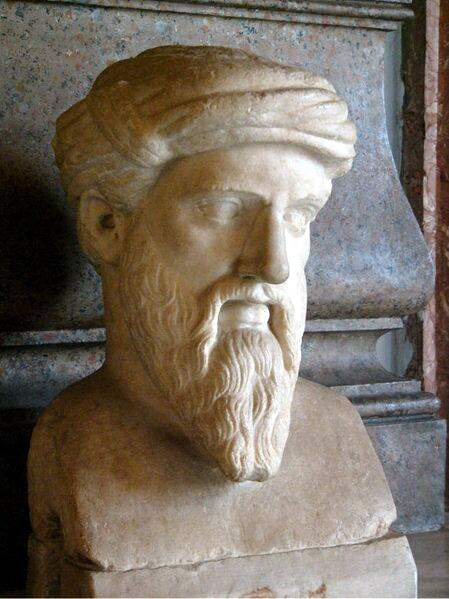
\includegraphics[height=0.7\textheight]{pythagoras}
  \par
  \vspace{4ex}
  Pythagoras would be proud.
\end{frame}

\section{Hardness Proofs in Coq}

\begin{frame}
  \frametitle{How do we define NP-hardness in Coq?}

  Formally, perhaps we should define NP-hardness starting from nondeterministic Turing machines...

  \pause
  \vspace{5ex}

  ...but that sounds difficult, so let's just use Karp reductions starting from a well-known NP-hard problem: FORMULA-SAT.
\end{frame}

\begin{frame}
  \frametitle{What is a Karp reduction?}
  \framesubtitle{And how do we prove one valid?}

  \onslide<4->{To prove} a Karp reduction $A \leq B$ is valid\only<-3>{ if it is}\only<4->{, we must}
  \vspace{3ex}

  \renewcommand{\arraystretch}{1.5}
  \begin{tabular}{rcc}
    & \onslide<5->{PL community?} & \onslide<7->{hardness community?} \\
    \textbf<9>{\onslide<4->{Prove} \onslide<2->{correct}\onslide<4->{ness}} & \textbf<9>{\action<5-|alert@5>{easy}} & \textbf<9>{\action<7-|alert@7>{hard}} \\
    \onslide<4->{Prove} \onslide<3->{polytime}\onslide<4->{ness} & \action<6-|alert@6>{hard} & \action<8-|alert@8>{easy} \\
  \end{tabular}
  \renewcommand{\arraystretch}{1}
\end{frame}

\begin{frame}[fragile]
  \frametitle{Encoding reductions in Coq}

  \begin{minted}{coq}
Class problem A :=
  { ProblemSize : A -> nat;
    ProblemYes : A -> Prop;
  }.
  \end{minted}

  \pause

  \begin{minted}{coq}
Class reduction `(PA : problem A)
                `(PB : problem B)
                 (f : A -> B) :=
  { ReductionPolytime : polytime f;
    ReductionCorrect : forall x,
        ProblemYes x <-> ProblemYes (f x);
  }.
  \end{minted}
\end{frame}

\begin{frame}
  \frametitle{The state of our reductions}

  \centering
  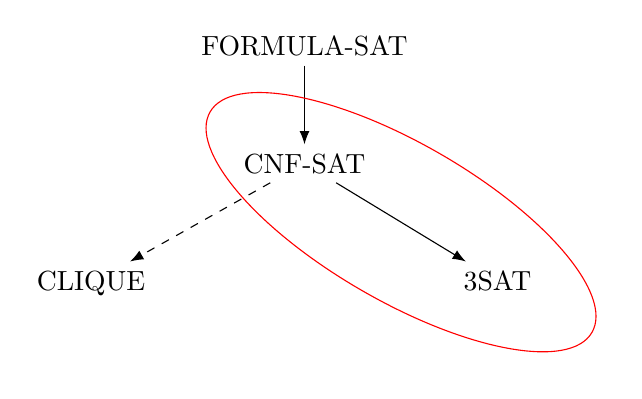
\begin{tikzpicture}
    \node (fs) {FORMULA-SAT};
    \node[below=of fs] (cs) {CNF-SAT};
    \node[below right=of cs] (ts) {3SAT};
    \node[below left=of cs] (cl) {CLIQUE};

    \draw[-Latex, visible on=<2->] (fs) -- (cs);
    \draw[-Latex, visible on=<3->] (cs) -- (ts);
    \draw[-Latex, dashed, visible on=<4->] (cs) -- (cl);

    \draw[red, rotate=60, visible on=<5->] ($(cs)!0.5!(ts)$) ellipse[x radius=1,y radius=2.8];
    %% \draw[red] (cs.north) to[closed,curve through={(cs.north west) .. (ts.south west) .. (ts.south east) .. (ts.north east) .. (cs.north east)}] (cs.north);
  \end{tikzpicture}
\end{frame}

\begin{frame}[fragile]
  \frametitle{CNF-SAT $\leq$ 3SAT}
  \framesubtitle{Definition of CNF-SAT}

  \begin{minted}[fontsize=\footnotesize]{coq}
Inductive literal :=
| PosLit : var -> literal
| NegLit : var -> literal
.

Definition clause : Type := list literal.
Definition cnf_formula : Type := list clause.
Definition assignment : Type := var -> bool.
  \end{minted}
\end{frame}

\begin{frame}[fragile]

  \begin{minted}[fontsize=\footnotesize]{coq}
Definition satisfies_literal (a : assignment) (l : literal) : bool :=
  match l with
  | PosLit v => a v
  | NegLit v => negb (a v)
  end.

Fixpoint satisfies_clause (a : assignment) (c : clause) : bool :=
  match c with
  | nil => false
  | l :: c' => satisfies_literal a l || satisfies_clause a c'
  end.

Fixpoint satisfies_cnf_formula (a : assignment) (f : cnf_formula) : bool :=
  match f with
  | nil => true
  | c :: f' => satisfies_clause a c && satisfies_cnf_formula a f'
  end.

Definition cnf_satisfiable (f : cnf_formula) : Prop :=
  exists (a : assignment), satisfies_cnf_formula a f = true.
  \end{minted}
\end{frame}

\section{Future Work}

\begin{frame}
  \frametitle{...and this}
\end{frame}

\end{document}

